% !TEX root = ../thesis.tex
\chapter{Behaviours of Evaluation Engines}
\label{sec:behaviours}

Based on the definitions in Chapter~\ref{sec:definitions} we will now look at different schedules of evaluation engines and compare them.
This is done in multiple steps: starting with a small subset of allowed schedules and functions and iteratively adding more complex cases.

For the comparision we will use timed transducers from Section~\ref{sec:definitions:timed_transducer}.
To do this the notion of a run of an evaluation engine is not sufficient: transducers describe a relationship between inputs and outputs, runs describe stepwise generation of internal and output events.
Therefore the \emph{behaviour} of a run is defined, which maps a run to relationship between inputs and outputs.

\begin{definition}[name = Behaviour of a Run]\label{def:behaviour_run}
  Let \(r\) be a run of an evaluation engine.
  The behaviour \(\beta_r\) of it is built stepwise:
  \begin{enumerate}
    \item Let \(\beta_r = \emptyset\)
    \item Take the prefix \(r_p\) of \(r\), where the first transition consumes an input upto but not including the next transition where an input is consumed.
    \item Select all output events \(O_1\), which are possible none, that are produced at any step in \(r_1\).
    \item Add the tuple \((e_1,O_1)\) to \(\beta_r\).
    \item Remove \(r_p\) from \(r\).
    \item Goto step 2 if \(r\) is not empty, else terminate.
  \end{enumerate}

  Stated simple the run is chopped into pieces, where each piece begins with the consumption of an input events and ends before the next input is consumed.
  Then all outputs produced in one piece is in a relation with the consumed input.
\end{definition}

The behaviour can be seen as a timed transducer since all events have timestamps and all consumed events are strictly ordered by their timestamp, since inputs to an evaluation engine are required to be ordered by their timestamp.

Since the behaviour encodes the relationship between inputs and outputs a run produces it provides the foundation to reason about equivalence between different runs and whole evaluation engines.

\begin{definition}[name=Equivalence of Runs]\label{def:equivalence_runs}
  Two runs are called equivalent if their behaviour is observational equivalent.
\end{definition}

Now we can define when two evaluation engines are called equivalent based on their runs

\begin{definition}[name=Equivalence of Evaluation Engines]\label{def:equivalence_eval_engine}
  Two evaluation engines are called equivalent, if for every run that one can produce there is an observational equivalent run in the other.
\end{definition}

\section{Schedules Without Timing Functions}
\label{sec:behaviours:without_timing}

For a first step we specify and compare behaviours of different approaches to evaluate \gls{tessla} specifications without timing functions.
Without timing functions all nodes work only on values or the presence of events and will emit exactly one event at every computation, either a normal or a progress event.
This leads to behaviours that can be easily reason about, as seen in the next sections.

All systems to evaluate \gls{tessla} specifications we will look at are based on the described structure in Section~\ref{sec:definitions:eval_engine}.
While there are other approaches to evaluation, a \gls{dag} based approach seems to fit most naturaly and focusing on one structure makes comparing systems easier.

Let's recap and summarize how an evaluation engine performs its computation.
Each evaluation engine will work in steps, where each step is synonymous with an index in the run of the system.
Therefore at each step one enabled node is scheduled to perform its operation, represented as the transition in the run.
The transition will encode one of the following three things that can happen:

\begin{itemize}
  \item The next external event (external events have to be totally ordered by their timestamp) can be consumed by a source in the \gls{dag}, which generates internal events, that are propagated to its children.
  \item An internal node, which has at least one new input buffered on all of its input queues, can perform its computation and generate a new internal event, which is propagated to the children of that node.
  \item An output node, which has at least one new input buffered on all of its input queues, can produce a new output.
\end{itemize}

Evaluation engines are free in the way they are scheduling their nodes, only limited by causality (no event can be consumed before it's produced), which is guaranteed by the enabledness criteria.
In the following evaluation engines are classified by their scheduling approaches.

\subsection{Greedy Evaluation Engines}
\label{sec:behaviours:without_timing:greedy}

The first class of evaluation engines are called greedy.

\begin{definition}\label{def:greedy_schedule}
  A schedule of an evaluation engine built by the following steps is called \emph{greedy}.
  \begin{enumerate}
    \item Select all nodes that are no sources, let their count be \(i\)
    \item Label them with unique natural numbers from \([1,i]\) in reverse topological order
    \item Label the remaining nodes with unique natural numbers bigger than \(i\)
    \item Schedule the enabled node with the lowest label first
  \end{enumerate}

  We also call an evaluation engine greedy if we mean it's run with a greedy schedule.
\end{definition}

Obviously for many \glspl{dag} there is no unique reverse topological order, therefore one can be chosen by the evaluation engine.
We will show in Section~\ref{sec:behaviours:equivalence_without_timing:greedy} that all topological orders will produce observational equivalent behaviours.

The greedy schedule ensures that no node is scheduled which has a successor that can be scheduled, therefore events are \emph{pushed} through the \gls{dag} towards an output node as fast as possible.
As shown in Section~\ref{sec:behaviours:without_timing:greedy:is_fair} any schedule built like this is fair.

Greedy evaluation engines offer a good start to reason about behaviours and will be used as a comparision for all other evaluation engines.

\begin{definition}[name = Valid Evaluation Engines]\label{def:valid_eval_engine}
  An evaluation engine is called \emph{valid} if it is equivalent to a greedy evaluation engine.
\end{definition}


\begin{figure}
  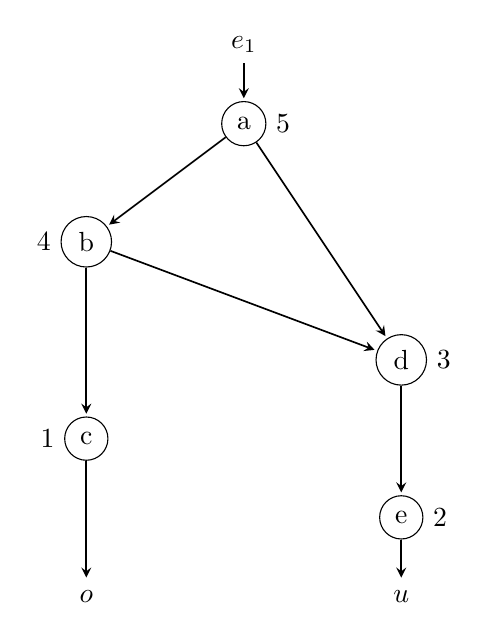
\begin{tikzpicture}
    [pre/.style={<-,shorten <=1pt,>=stealth,semithick}]
    \node (s) at (2,5) {\(e_1\)};
    \node [shape=circle,draw=black] (a) [label=right:5] at (2, 4) {a}
      edge [pre] (s);
    \node [shape=circle,draw=black] (b) [label=left:4] at (0,2.5) {b}
      edge [pre] (a);
    \node [shape=circle,draw=black] (c) [label=left:1] at (0,0) {c}
      edge [pre] (b);
    \node [shape=circle,draw=black] (d) [label=right:3] at (4,1) {d}
      edge [pre] (a)
      edge [pre] (b);
    \node [shape=circle,draw=black] (e) [label=right:2] at (4,-1) {e}
      edge [pre] (d);
    \node (o1) at (0,-2) {\(o\)} edge [pre] (c);
    \node (o2) at (4,-2) {\(u\)} edge [pre] (e);
  \end{tikzpicture}
  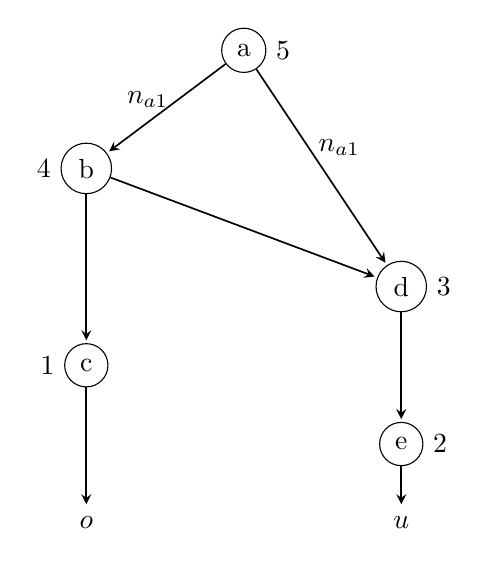
\begin{tikzpicture}
    [pre/.style={<-,shorten <=1pt,>=stealth,semithick}]
    \node [shape=circle,draw=black] (a) [label=right:5] at (2, 4) {a};
    \node [shape=circle,draw=black] (b) [label=left:4] at (0,2.5) {b}
      edge [pre] node[align=left,left,pos=0.6] {\(n_{a1}\)} (a);
    \node [shape=circle,draw=black] (c) [label=left:1] at (0,0) {c}
      edge [pre] (b);
    \node [shape=circle,draw=black] (d) [label=right:3] at (4,1) {d}
      edge [pre] node[align=right,right,pos=0.6] {\(n_{a1}\)} (a)
      edge [pre] (b);
    \node [shape=circle,draw=black] (e) [label=right:2] at (4,-1) {e}
      edge [pre] (d);
    \node (o1) at (0,-2) {\(o\)} edge [pre] (c);
    \node (o2) at (4,-2) {\(u\)} edge [pre] (e);
  \end{tikzpicture}
  \caption{Visualization of a simple evaluation engine with a greedy schedule.}
\label{fig:chap5:sec_greedy:visual_dag}
\end{figure}

Figure~\ref{fig:chap5:sec_greedy:visual_dag} visualizes a greedy evaluation engine.
It shows two \glspl{dag} representations of an evaluation engine  where the nodes \(a\) to \(e\) are labeled in a reversed topological order and \(o\) and \(u\) represents two output streams.
The left system is in its initial state and an input event \(e_1\) is present and can be consumed by the input node \(a\).
When a node is chosen to compute by the scheduler, only node \(a\) is enabled, therefore it is scheduled.
The right system is the representation of the next step: node \(a\) has consumed the external event and produced an internal event \(n_{a1}\), which is propagated to all its children: nodes \(b\) and \(d\).
In the next step node, \(b\) would be scheduled, because it has the lowest number of any node that can compute (actually it's the only node that can compute at all, because \(d\) has to wait for the event from \(b\)).
After \(b\) is scheduled, it would produce the internal event \(n_{b1}\) which would then be distributed to nodes \(c\) and \(d\).

The complete run of the greedy engine for one input is the following, where the states are omitted:

\begin{align*}
  \langle
    (\lambda,                             s_0),
    ((\{ n_{a1}         \}, \{n_{b1}\}),  s_1),
    ((\{ n_{b1}         \}, \{o_1\}),     s_2),\\
    ((\{ n_{a1}, n_{b1} \}, \{n_{d1}\}),  s_3),
    ((\{ n_{d1}         \}, \{u_1\}),     s_4)
  \rangle
\end{align*}

If there were more than one input event, at this point node \(a\) would be scheduled again.
It would consume the next external event and the following nodes would be scheduled in the same order as before, extending the run in an obvious way.

\subsubsection{Fairness of Greedy Schedules}
\label{sec:behaviours:without_timing:greedy:is_fair}

It remains to show that greedy schedules are fair.

\begin{lemma}[name = Greedy Schedules are Fair]\label{lemma:greedy_schedules_are_fair}
  Any greedy schedule is fair.
\end{lemma}

\begin{proof}
  Let \(a\) be a node with the label \(n\), which is enabled at step \(i\) and is no source.
  Because evaluation engines can only contain a finite number of nodes there can only be a finite number of enabled nodes with a smaller label than \(n\).
  Furthermore all nodes can only have a finite number of events buffered, since all nodes can only produce a finite number of events per computation and therefore only a finite number of events can be produced after a finite number of steps.
  Therefore after a finite number of steps \(j\) all nodes with a smaller label than \(n\) will be disabled.
  The only way new events could enter the system are through sources, but they have bigger labels than \(n\), as by the definition of the schedule, and therefore can't be scheduled before \(n\).
  Because of Lemma~\ref{lemma:enabled_till_scheduled}, \(a\) will still be enabled after these steps.
  So \(a\) is the enabled node with the lowest label at step \(i + j\) and therefore will be scheduled.

  Now let \(a\) be a source.
  Sources are only scheduled when no internal node is enabled since they are labeled with higher numbers than all internal nodes.
  Based on the same reasoning as in the first case at some point all internal nodes will become disabled, therefore a source node has to be scheduled.
  This source can either be \(a\) or another source, recall that only one source is enabled at any time because of the environment of an evluation engine.
  If another source was scheduled, after a finite amount of steps all internal nodes will have to become disabled again.
  Since finite traces are evaluated at some point either the trace will end without ever feeding an input to \(a\), then \(a\) will never be enabled, or at some point \(a\) will receive an external event.
  When \(a\) receives an external event, it will be the only enabled source, else no input would be fed to an input at that step.
  Therefore \(a\) will be scheduled the next time no internal nodes are enabled.
\end{proof}


\subsection{Fair Evaluation Engines}
\label{sec:behaviours:behaviour_without_timing:fair}

Obviously greedy schedules are only a small subset of all fair schedules.
As the next step we will look at the rest of them.

\begin{definition}[name = Fair Evaluation Engines]\label{def:fair_evaluation_engines}
  A fair evaluation engine is one with a fair schedule.
\end{definition}

In contrast to a greedy evaluation engine a fair one has no fixed schedule, meaning that at each step any enabled node can be scheduled.
Therefore predecessors of enabled nodes can perform multiple computations before their children are scheduled and events are not \emph{pushed} through the \gls{dag} as fast as possible.

The difference between greedy and fair schedules are similar to the ones of synchronous and asynchronous transducers: A greedy schedule will ensure that outputs are produced as fast as possible while a fair can \emph{delay} the outputs by consuming multiple inputs first and scheduling internal nodes multiple times before scheduling an output node.
But note that there is an important difference between synchronous transducers and the behaviour of a greedy evaluation engine: A greedy evaluation engine can consume multiple events and produce multiple events at every step, as it may have multiple sources and multiple outputs.

\section{Equivalence of Different Schedules Without Timing Functions}
\label{sec:behaviours:equivalence_without_timing}

The behaviour of a run of an evaluation engine with a given schedule allows us to reason about equivalence.

As defined by definition~\ref{def:valid_eval_engine} any evaluation engine has to be equivalent to a greedy one to be valid.

The equivalence is shown in two steps: first in Section~\ref{sec:behaviours:without_timing:greedy} it is shown, that all possible greedy engines for a specification are equivalent, so there is only one valid evaluation for a specification over a fixed input.
Afterwards in Section~\ref{sec:behaviours:equivalence_without_timing:greedy_fair} it is shown that any fair evaluation engine is equivalent to a greedy one.


\subsection{Equivalence of Greedy Systems}
\label{sec:behaviours:equivalence_without_timing:greedy}

When given a series of input events, two greedy evaluation engines for a specification with different schedules will have different runs.
But both will produce all outputs that can be produced after consuming one specific input before the next input is consumed as reasoned in Section~\ref{sec:behaviours:without_timing:greedy}.
Also both runs will obviously have the same length (both engines are the same \gls{dag}, so they have the same number of nodes), let that length be \(l\).

To proof the equivalence of both engines we can prove the equivalence of their runs.
To show the equivalence we will show that there is always another run, which is equivalent to the second one, that is closer to the first one.
If such a closer run always exist, we will show that the run with closeness \(l, 0\) to the first run, which has to be the first run itself, is also an equivalent run to the second run.

\begin{theorem}[name = Equivalence of Different Greedy Evaluation Engines]\label{theorem:equivalence_greedy_eval_engines}
  Two greedy evaluation engines for a specification with different schedules are equivalent.
\end{theorem}

\begin{proof}

  todo reason based on behaviour.
  Let \(r_1, r_2\) be the runs of the two engines for a given \gls{tessla} specification.
  Because each \gls{tessla} specification contains only a finite amount of functions and works on finite traces, the runs also have to be finite.

  If the two runs aren't equal, they must have a closeness which is smaller than \((l, 0)\).
  Let \([r_2]\) be the set of all runs that are equivalent to \(r_2\).
  All of those runs will also have a closeness from \(r_1\) which is smaller than \((l, 0)\).
  Select one run \(r_2' \in [r_2]\) which has a minimal closeness from \(r_1\).
  Let \((d,k) = \delta(r_1, r_2')\).

  This means that at step \(d\) the run \(r_2'\) has taken a different transition than run \(r_1\).
  Let the transitions the runs have taken be \(\tau_1\) for \(r_1\) and \(\tau_2\) for \(r_2'\).
  Run \(R_2'\) will take transition \(\tau_1\) at step \(d+k\) (as per the definition of the closeness).
  Obviously the two transitions have to be independent of each other, else they couldn't have been taken in different order by the two runs.

  If \(k > 1\) there will be a transition \(\tau_2' \neq \tau_1\) which is taken by the run \(r_2'\) at step \(d+(k-1)\).
  While this transition \(\tau_2'\) must also be taken in the first run as per Lemma~\ref{lemma:enabled_till_scheduled}, it's not possible, that it was taken before \(\tau_1\), beause then the two runs wouldn't have been the same upto the point where \(\tau_1\) was taken.
  Therefore \(\tau_1\) has to be independent of \(\tau_2'\), and because \(\tau_2'\) was scheduled by the second run before \(\tau_1\) both transitions are independent of each other.

  As of Lemma~\ref{lemma:exchange_independent_transitions} which one of them is taken first can't change the enabledness of the node of the second transition.
  Therefore there is a run \(r_2''\), which is equal to \(r_2'\), except that the transitions \(\tau_1, \tau_2'\) are scheduled the other way around.
  Therefore the runs \(r_2'\) and \(r_2''\) are equivalent and their closeness to \(r_1\) is \(d, k-1\), which contradicts the initial statement that \(r_1'\) was a run with a maximal closeness.
  This means that there is an equivalent run to \(r_2\) which has at least the closeness \((d, 1)\).

  If \(k = 1\) the transition \(\tau_2'\) from the previous case is equal to \(\tau_2\).
  Based on the same reasoning there also exist a run \(r_2''\) which is equal to \(r_2'\), except that the order of \(\tau_2\) and \(\tau_1\) is changed, and which is also equivalent to \(r_2'\) and to \(r_2\).
  This run has the closeness \((d, 0)\) to \(r_1\).
  This obviously doesn't make sense: The first element of the closeness is the last step where both runs are equal, the second element describes how many steps afterwards the differing transition was taken.
  But if it was taken right in the step after the last equal step, there is no difference at that position, so the closeness of \(r_1\) and \(r_2''\) can be at least \((d+1, x), x \in \mathbb{N}_{>0}\).
  This also contradicts our initial statement that \(r_2'\) was the run with the biggest closeness to \(r_1\) which is equivalent to \(r_2\).

  Combined we can now say, that there is no upper bound on the closeness of equivalent runs of \(r_2\) to \(r_1\), therefore the run with the closeness \((l, 0)\) also has to be equivalent to \(r_2\).

\end{proof}

\subsection{Equivalence of Greedy and Fair Evaluation Engines}
\label{sec:behaviours:equivalence_without_timing:greedy_fair}

When the nodes of \(a\) aren't scheduled in reversed topological order, the system can consume inputs before producing all outputs based on the last consumed input.
Therefore the reordering of runs has to be performed over wider parts of the run.
% Idea: each step is a commutation of two internal events in regard to the rev top order.
% => show commutativity of traces (note: only valid commutations, no two events, where one depends one the other, can be commuted, this is ensured by the scheduling of nodes that have input buffered)

\section{Behaviour with Timing functions}
\label{sec:behaviours:with_timing}
\section{Equalitys with Timing functions}
\label{sec:behaviours:with_timing}
\section{Parallel computation}
